\documentclass[aps,pra,preprint,groupedaddress]{revtex4-1}
<<<<<<< HEAD
%\documentclass[aps,prl,preprint,superscriptaddress]{revtex4-1}
%\documentclass[aps,prl,reprint,groupedaddress]{revtex4-1}
=======
>>>>>>> 374802a66b0f5e758bfa0525da6bb1c6ef6512f6

\usepackage{graphicx}
\usepackage{amsmath}

\begin{document}

\title{Phase Dependent Ionization of Rydberg Atoms in Static Fields}

\author{Eric Magnuson}
\email[]{edm5gb@virginia.edu}
\author{Tom Gallagher}
\affiliation{University of Virginia, Department of Physics}

\date{\today}

\begin{abstract}
Pump-probe schemes using high frequency pulsed light synchronous to strong field low frequency fields are a prolific tool for probing atomic, molecular and surface electron dynamics. We realize one such system in Rydberg states of Li using an 819-nm excitation laser amplutde modulated synchronously to a 15.9-GHz microwave field. We show that when the modulation is at the same frequency of the microwave field, phase dependent ionization is only observed in the presence of static fields. Our results are well described by a computational model. Analysis of this model shows the importance of multiple classical electron orbits.
\end{abstract}

\maketitle

\section{\label{sec:intro}Introduction}

Attosecond-IR experiments very useful. Test understanding of ionization in strong-field + Coulomb regime. High-harmonic-generation. Attosecond streaking to use strong fields to get time-resolved electron dynamics, ultrafast chemistry, and probe internal structure of large atoms / molecules.

The techniques and principles of attosecond-IR experiments have more broad appeal. THz experiments w/ pulsed ps, fs or as lasers use similar concepts experimental principles. Past work has extended this to application in Rydberg atoms using MW fields and pulsed excitation lasers. Shown phase dependent ionization, provided tool for probing the dynamics of Rydberg electrons near the ionization limit.

We now show the effect of breaking symmetry of system by adding pulsed electric field during excitation. Comparable to symmetry arguments used in THz and Attosecond experiments.

We provide further improvements to the computational model.


\section{\label{sec:back} Background}

Qualitatively describe behavior of electrons near ionization limit in MW fields, and recent work (Alexandr). Rydberg states with long lifetimes in strong MW field. Long orbits.

Include simpleman's + coulomb model discussed in Shuman and Overstreet. Maximum energy exchange at what phase? Describe qualitatively the process this model describes: Electron leaves core exchanging energy w/ MW field. Goes on an orbit in the static field that either ionizes or doesn't. Returning to the core, the electron can exchange energy again, the process repeats. Long orbits protect bound states from returning and maybe getting ionized.

(MAYBE) show how these calculations give a $\Delta E$ vs $\phi_0$ for initially leaving the core, and a return.

Show that when probing with a amplitude modulated laser, the observations can only be at the modulation frequency.

Show that symmetry arguments limit what harmonics of the MW field the system response can include.

(MAYBE) Show that if we limit system response to what initial energy transfer happens, this limits the phase of the phase-dependent signal to particular phases ($7\pi/6$ and $\pi/6$ in static fields, ($\pi/6$ and $7\pi/6$) or ($4\pi/6$ and $11\pi/6$) in zero field.

\section{\label{sec:exp} Experimental Methods}

Note: \emph{INCLUDE LEVEL DIAGRAM}

In this experiment, Li atoms in a collimated thermal beam are optically excited to high lying Rydberg or continuum states along the path $2s \xrightarrow{\text{671 nm}} 2p \xrightarrow{\text{610 nm}} 3d \xrightarrow{\text{819 nm}} nf, \epsilon f$. These optical beams intersect at a right angle forming a rectangular 1 mm$^3$ excitation region. This region is at an anti-node of a 15.9 GHz Fabry-Perot microwave cavity. The excitation occurs in the presence of microwave fields, so that the $nf, \epsilon f$ electron exchanges energy with the field as it leaves the atomic core.

The microwave cavity is allowed to load for 240 ns before the first laser pulse, and the microwave input is shut off 20 ns after the last laser pulse, allowing the cavity to empty. Synchronous with the MW power envelope, a static field pulse is applied to the top and bottom aluminum plates to produce a vertical static field in the interaction region. The 610-nm and 671-nm lasers are pulsed synchronously for 20 ns, after which the 819-nm laser is pulsed with a square envelope for 20 ns. One microsecond after the last laser pulse, we field ionize surviving Rydberg states within 100 GHz of the ionization limit by applying a negative voltage pulse to an aluminum plate below the interaction region. Ionized electrons are pushed into a microchannel plate (MCP) assembly which produces a voltage pulse proportional to the number of electrons detected. This pulse is integrated through a boxcar integrator and recorded.

The signal detected is normalized to the signal from the total number excited electrons. The total excitation ($S_{total}$) is measured by applying the field ionization pulse during excitation, so all Rydberg and continuum states are driven to the detector. This value is compared to the signal observed when the field ionization pulse occurs 1 $\mu$s after the final laser pulse, which only detects bound Rydberg states $S_{Ryd}$. Signals reported in this paper always show $S = S_{Ryd} / S_{total}$.

\begin{figure}
	\includegraphics[width=0.7\textwidth]{fields}
	\caption{Temporal view of the microwave field (top) phase-locked with the amplitude modulated laser intensity (bottom). The peak laser intensity occurs at the phase $\omega t_0$ of the microwave field, and can be adjusted by an optical delay line.}
	\label{fig:AMLaser}
\end{figure}

Probing phase dependence in this experiment is achieved by synchronizing the amplitude modulation of the 819-nm laser to a microwave field in the cavity, as shown in Fig.~\ref{fig:AMLaser}. The laser field can be described by an envelope modulating a fundamental frequency:
\begin{equation}
E_{opt}(t) = E_o \sin{(\omega_o t)} \cos{(\omega(t-t_0))}
\end{equation}
The 
Using an optical delay line, the phase of the modulation envelope of the 819-nm laser can be delayed relative to phase of the microwave field. This modulation is proportional to the excitation-rate to a Rydberg or continuum state, so delaying the modulation envelope is equivalent to changing the phase $\omega t_0$ of the microwave field at which excitation occurs.

\subsection{\label{sec:dye} Dye Lasers}

We use two dye lasers at 670-nm and 610-nm to drive the $2s \rightarrow 2p$ and $2p \rightarrow 3d$ transitions, respectively. These dye lasers are pumped by a Quantronix Darwin Nd:YLF. The pump laser produces 30-W, approximately 100-ns FWHM pulses at a 1-kHz repetition rate. Using a Pockels cell (PC) and polarizing beam splitter (PBS), the rising edge of the pulse is picked off and split equally between to the 670-nm and 610-nm lasers. A second PC and PBS directs a 20-ns slice from the peak of the pump pulse to a dye amplifier for the 819-nm laser. The long trailing edge of the pump pulse is dumped.

The 670-nm dye laser uses a Littman-style cavity and LDS-698 laser dye dissolved in Ethanol as a lasing medium. The 610-nm uses a H{\"a}nch style cavity with Rhodamine-610 laser dye dissolved in Ethanol. Both lasers have an approximate FWHM of 10-GHz. To minimize unintended ionization from the $3d$ state, both lasers are attenuated to 2 $\mu J$ pulses before being directed to the vacuum chamber.

\subsection{\label{sec:ampmod} Amplitude Modulated 819 nm Laser}

\begin{figure}
	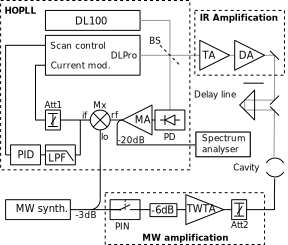
\includegraphics[width=0.7\textwidth]{beatexp}
	\caption{Schematic showing how the amplitude modulated laser is produced, locked to the microwave frequency, and how both the laser and microwave fields are delivered to the interaction region. The AM IR laser is generated by overlapping the DL-Pro and DL-100 laser beams on a beamsplitter (BS). One output is amplified and sent to the interaction region. The microwave field is generated by a synthesizer, formed into pulses by the PIN switch and amplified by the Traveling Wave Tube Amplifier (TWTA) before injection into the microwave cavity. The locking of the IR intensity envelope to the microwave field is performed by the Heterodyne Optical Phase Locked Loop (HOPPL).}
	\label{fig:pll}
\end{figure}

Fig.~\ref{fig:pll} shows how the amplitude modulated laser and microwave fields are produced and delivered to the interaction region, and how they are locked in a phase locked loop. The 819-nm laser is produced from two external-cavity diode lasers, a Toptica DL-100 and DL-Pro. The lasers are tuned such that their frequencies are separated by the microwave frequency, and the two beams are overlapped on a 50:50 beamsplitter (BS). This overlapping produces a beat-note in the laser intensity at the microwave frequency. One output from the beamsplitter is directed to a high speed photodetector that can detect the beat note and deliver the signal to the phase-locked-loop. The second output from the beamsplitter is directed through an amplification chain and to the interaction region.

The amplitude modulation of the laser is locked to the microwave frequency with a heterodyne optical phase-locked-loop (HOPLL). The locking is driven by a "fast" feedback to the current input of the DL-Pro, and a "slow" feedback to the scan input. To produce an error signal, the amplitude modulation is detected after the 50:50 beamsplitter by a fast photodiode. The DC signal is filtered out, leaving only the AC component. This is amplified and mixed with the microwave source to produce an error signal. The error signal is passed through a variable attenuator and then connected to the Current input of the Toptica DL-100. This achieves a lock between the laser ampltude modulation frequency and the microwave field that lasts for several minutes.

To achieve longer lock times on the order of hours, we use a Toptica PID-110 to drive the scan input of the DL-Pro. The "fast" current lock is primarily lost due to the lasers drifting past the range that the current input can correct. Low-frequency components of the error signal are processed through a PID and fed to the Scan input. This corrects long term drifts in the amplitude modulation frequency, leaving only high-frequency errors for the "fast" loop to correct.

The second output of the 50:50 beamsplitter produces 30 mW of aplitude modulated light. This is passed through a tapered amplifier and a dye amplifier. The Toptica Tapered Amplifier increases the continuous beam power to 800 mW. The dye amplifier is pumped by a 20-ns square pulse picked from the peak of the Nd:YLF laser pulse. We use LDS-819 dissolved in Ethanol as the amplfication medium. This produces a 20 ns long, 6 $\mu$W pulse of amplitude modulated 819-nm light.

Once locked, the AM phase at the BS is constant relative to the MW phase, and their relative phase in the interaction region depends only on the effective path length difference. To adjust the path length of the AM laser beam, after amplification the beam is passed through an optical delay before continuing to the interaction region. This optical delay consists of a retro-reflector mounted to a translation stage, able to extend the path length of the AM laser by several MW wavelengths.

\subsection{\label{cavity} Microwave Apparatus}

A Hittite HMC T-2100 synthesizer tuned to the 15.9-GHz resonance of the microwave cavity is used as our microwave source. The Hittite produces 9 dBm, and a splitter diverts half of the power to the microwave mixer to generate the error signal for the PLL. The other half of the signal is formed into 300-ns pulses by a microwave switch, and then amplified by a Hughes 8020H04F traveling-wave-tube-amplifier (TWTA). Between the TWTA and the cavity, there is a 0 to 50 dBm variable attenuator allowing us to control the intensity of the pulse incident on the microwave cavity.

The microwave cavity is a Fabry-Perot cavity composed to two brass spherical mirrors. These mirrors have a radius of curvature of 10 cm and are 10.2 cm in diameter, with an on axis separation of 7.83 cm. The 15.9 GHz resonance is the TEM$_{008}$ mode of the cavity, with a quality of 3600. We are able to determine the field inside the cavity to \emph{15\%}.

\subsection{\label{fields} Static Fields}

This experiment depends on the detection of long lived Rydberg states close to the ionization limit. To prevent these states from ionizing before detection, we must minimize the persistent static field in the interaction region. We accomplish this by surrounding the interaction region on two sides with the brass microwave cavity mirrors, and on the remaining two sides, top, and bottom with polished aluminum plates. A voltage can be applied independently to each plate or mirror, allowing us to compensate persistent static fields in every direction. We measure the depressed ionization limit (DIL) to minimize stray fields and estimate the residual persistent static field. In this manner, we determine the remaining persistent static field to have a magnitude of 1.5 mV / cm. This results in a DIL of 7 GHz below the the zero field ionization limit. This value for the DIL is constant in all future experiment and discussion in this paper.

To observe phase dependent ionization, we apply a pulsed vertical static field to the interaction region during excitation of Rydberg states. This is done using a two-channel arbitrary waveform generator (AWG) to apply 300-ns square pulses of opposite magnitudes to the top and bottom bias plates. This square pulse is synchronous with the microwave pulse, the leading edge arriving 240-ns before the first laser pulse and the trailing edge arriving 20-ns after the end of the 819-nm laser pulse. Turning off the applied static field minimizes the static field ionization of the high-lying states we wish to observe. 1 $\mu s$ after the final laser pulse, the same AWG applies a voltage to the bottom plate to produce a -0.65 V / cm ionization field, ionizing high-lying states and pushing ionized electrons toward the MCP stack.

\section{\label{results} Results}

\begin{figure}
	\includegraphics[width=0.7\textwidth]{phase_delay}
	\caption{Rydberg state signal as the phase delay is scanned. The central laser frequency $2\pi\omega_0$ is tuned to 2 GHz above the DIL. The vertical scale is normalized such that 1 is the total number of electrons excited by the 819 nm laser. When no pulsed field is applied, there is no observed phase modulation. As the pulsed field in increased,  phase dependence in the signal grows and then lessens as the total mean signal decreases. Grey shows the experimental data, while the solid sinusoidal curves trace the best fit to Eq.~\ref{eq:modfit}.}
	\label{fig:phase_delay}
\end{figure}

Fig.~\ref{fig:phase_delay} shows that, when the laser intensity is modulated at the same frequency as the microwave field, a phase dependent ionization can only be observed when a static field is present during excitation. The central frequency of the excitation laser is tuned to 14 GHz below the DIL (21 GHz below the zero-field ionization limit), in the presence of a 4 V/cm microwave field. The optical delay $\omega t_0$ is scanned while measuring the Rydberg signal. The signal is normalized to the total excitation. Results are shown for $E_{pulse} =$ 0, 7.2, 36.0 and 108.0 mV/cm. At zero field, there is no observed phase dependence, while at 7.2 mV/cm the phase dependent signal is modulated by 5\% of the total excitation. This agrees with the prediction that phase dependent ionization can only be observed at the microwave field frequency when a static field is applied to lift the vertical symmetry of the system. As $E_{pulsed}$ is increased further, we see both the mean signal and the peak to peak modulation decrease. Though the delay at which the detected signal is greatest shifts somewhat at higher pulsed field, for fields in the $+\hat{z}$ direction, we observe peak signal near $7\pi/6$, and a minimum near $\pi/6$.

We quantify these observations by fitting the signal vs. delay to a sinusoidal model:
\begin{equation} \label{eq:modfit}
S = A \cos{[\omega t - \phi_0]} + S_0
\end{equation}
The model frequency is fixed at $\omega = 2\pi / f_{MW}$, while the amplitude (A), phase offset ($\phi_0$) and mean signal ($S_0$) are used as fit parameters. Using this model to quantify the phase-dependent Rydberg signals, we verify that phase dependent signals only occur in the presence of a vertical pulsed field, and are not observable in a horizontally pulsed field. In a 4 V/cm MW field and a 14 mV/cm pulsed field, we excite electrons with the AM-IR laser tuned 14 GHz below the DIL. The angle of the applied pulsed field relative to the MW field and IR laser polarization is adjusted using the bias plates around the interaction region.

\begin{figure}
	\includegraphics[width=0.7\textwidth]{circle_static}
	\caption{With the central IR frequency $2\pi\omega_o$ tuned to 14 GHz below the DIL, the angle above the horizontal of a 14.4 mV/cm pulsed field is rotated by applying pulsed voltages to vertical and horizontal bias plates. When the pulsed field is perpendicular to the vertical MW and IR polarization, there no phase dependence. The phase dependence grows as $\vec{E}_{pulsed}$ is rotated to have a larger vertical component. The measurement is repeated in three sets, and linear regression on the combined data set shows the peak to peak modulation crosses zero at $6.0 \pm 0.9$ degrees. This corresponds to $\vec{E}_{pulsed} \cdot \hat{z} = 1.5 \pm 0.2$ mV/cm, which is the approximate size of our stray static field.}
	\label{fig:CircleStatic}
\end{figure}

Fig.~\ref{fig:CircleStatic} shows the effect of applying a pulsed field at angles near perpendicular to the MW and IR polarization. The measurement was repeated three separate times, Each set of data showing the peak to peak modulation crosses zero when $\vec{E}_{pulse}$ is nearly horizontal, and has a linear relationship with the z-component of the field. A fit to all three sets of data shows modulation is zero at $6.0 \pm 0.9$ degrees below the horizontal, corresponding to a $-1.5 \pm 0.2$ mV/cm z-component of the pulsed field. This is explainable by the $<2$ mV/cm residual static field in the interaction region. As the angle is changed, the amplitude of the phase dependence increases linearly with the component of the pulsed field along the MW and AM laser polarization. This indicates that the static field in the polarization direction is required to break the symmetry of the system and observe phase dependence.

	\includegraphics[width=0.7\textwidth]{ModvsField}
	\caption{Mean signal ($S_0$) and peak-to-peak modulation ($2\cdot A$) against applied pulsed static field for excitation laser central frequencies of +2 GHz, -14 GHz, and -30 GHz relative to the DIL. A negative peak-to-peak modulation indicates the greatest Rydberg signal is detected with an optical delay near $\omega t_o = 7\pi/6$, while a negative modulation indicates the detected signal is greatest near $\omega t_o = \pi/6$.}
	\label{fig:ModvsField}
\end{figure}

With $\vec{E}_{pulse}$ parallel to $\hat{z}$, we explore how the fit parameters in Eq~\ref{eq:modfit} changes as the AM IR laser is tuned above and below the DIL at various field strengths. Fig.~\ref{fig:ModvsField} shows plots of both peak-to-peak phase dependence in the signal ($2\cdot A$) as well as mean signal ($S_0$) as a function of applied pulsed static field at 3 different laser tunings, DIL + 2, -14, and -30 GHz. For all three laser tunings, the mean signal behaves as expected. The signal is largest when there is no static field applied, and the high lying states we detect are longer lived. As the magnitude of the applied static field increases, mean signal monotonously decreases as the high lying states are more likely to ionize. The further below the DIL the central frequency of the excitation laser is tuned, the more slowly $S_0$ drops off with field.

The observed behavior of the peak-to-peak modulation is more complex. Fig.~\ref{fig:ModvsField} (a) shows observations with a laser tuning 2 GHz above the DIL. As shown in Fig.~\ref{fig:ModvsField}, at zero static field the symmetry of the system is not lifted and we cannot observe phase dependence. As the static field magnitude is increased phase dependence quickly emerges, reaching a maxima of peak-to-peak amplitude at 10 mV/cm. Then, as the total signal approaches zero, so does the modulation. In these figures, the peak to peak amplitude $2 \cdot A$ is positive if $\phi_0 \approx 7\pi/6$, and negative if $\phi_0 \approx \pi/6$. Because the applied static field is the only parameter lifting the vertical symmetry, applying an inverse static field produces inverse phase dependence. This shows in the peak-to-peak modulations at opposite applied static fields being approximately equal and opposite, corresponding to peak signal occurring at optical delays separated by $\Delta \omega t_0 = \pi$.

In Fig.~\ref{fig:ModvsField} (b), showing the AM IR laser tuned 14 GHz below the DIL, the behavior is more complex. Like the DIL + 2 GHz case, the peak to peak signal quickly increases as the pulsed field is increased from zero, reaching a peak near 10 mV/cm. However, the maximum field ionization signal occurs at a delay $\phi_0 = \pi/6$, rather than $7\pi/6$ as observed in the DIL + 2 GHz case. As the pulsed field is increased, the modulation falls, crossing through zero at 25 mV/cm, and then reaching a peak at 50 mV/cm with a positive amplitude matching the Fig.~\ref{fig:ModvsField} (a), representing $\phi_0 \approx 7\pi/6$.

Finally, Fig.~\ref{fig:ModvsField} (c) shows the case for the central AM IR frequency tuned to DIL - 30 GHz. This resembles the DIL - 14 GHz case in Fig.~\ref{fig:ModvsField} (b), except that the modulation appears to turn on at a non-zero pulsed field. Rather than immediately growing as the pulsed field is increased, the modulation doesn't start growing until $E_{pulsed} = \pm 20$ mV/cm. We attribute this to only a small window of phases allow either uphill or downhill to gain enough energy to ionize at small pulsed field. Thus the modulation doesn't start to rapidly increase until the depressed potential barrier seen by downhill electrons is pushed closer to $W_0$, at which point the system starts to more closely resemble Fig.~\ref{fig:ModvsField} (b).

\section{\label{sec:disc} Comparison to Computational Model}

\emph{To understand the experimental results shown in the previous section, we conduct two calculations of classical electron motion in the combined Coulomb, MW and pulsed field.}

\emph{The classical picture can be divided into three steps.}

\emph{1) Exchange energy with the MW field as it leaves the ion core.}

\emph{2) Undergo a long orbit. High energy electrons may ionize. Low energy electrons will return to the core while the pulsed and MW field are still on. Electrons in narrow energy band will undergo long bound orbits that do not return to the core until after the fields are zeroed.}

\emph{3) Electrons that return to the core will again exchange energy with the MW field as they slingshot around the ion core.}

\emph{Our first computation explicitly separates these stages. As a conceptual tool, we use a 1-D model to calculate the classical period of the orbit after the electron has exchanged energy with the MW field.}

\emph{Our second computation uses a 2-D model to continuously integrate the electron equations of motion until the static field has turned off and the MW field has rung down.}

\subsection{1-D Model and Turning Time}

\begin{figure}
	\includegraphics[width=\textwidth]{EvP}
	\caption{Energy exchange ($\Delta W_{MW}$) with the MW field vs. phase ($\omega t_0$) of the MW field at excitation for an electron leaving the ion core. Calculated by integrating the 1-D classical equations of motion for an electron initially excited with an orbital energy $v^2/2 - 1/r = 0$, starting from the inner turning point for an electron f-state angular momentum, $\approx 6$ a.u.. The calculated values for MW field amplitudes of 2, 4, and 6 mV/cm (color) fit closely to predicted values of $E_{MW} / \omega^{2/3} \cdot \cos(\omega t_0 - \pi/6)$ (black).}
	\label{fig:EvP}
\end{figure}

\begin{figure}
	\includegraphics[width=\textwidth]{up_and_down_orbits}
	\caption{The fate of an electron after it's first orbit. The y-axis is the $e^-$ orbital energy $W_{orbit} = W_0 + \Delta W_{MW}$ after exchanging energy with the MW field, and the x-axis shows the strength of $E_{pulsed}$. \textbf{Uphill Electrons:} \textbf{(a)} High energy $e^-$ in low field will directly ionize. \textbf{(b)} $E_{pulse}$ shuts off near the apoapsis of the $e^-$ orbit, and is left in a bound long-period orbit. \textbf{(c)} $E_{pulse}$ shuts off as the $e^-$ is returning to the core with positive orbital energy. It will swing around the core as the MW field rings down and ionize. \textbf{(d)} Low energy $e^-$ in high field orbits return to the core before $E_{pulse}$ or $E_{MW}$ turn off at 20 ns. The electron exchanges energy with the MW field at every return to the core, resulting in a random walk in energy that may result in ionization or remaining bound. \textbf{Downhill Electrons:} \textbf{(a)} High energy $e^-$ in small field will directly ionize. \textbf{(b)} At 20 ns the $e^-$ is near it's apoaxis and will be left in a long-period bound orbit. \textbf{(d)} The $e^-$ returns to the core before 20 ns and undergoes a random energy walk. Whether the final state is bound after many orbits is probabilistic.}
	\label{fig:orbits}	
\end{figure}

\begin{figure}
	\includegraphics{W0_2D}
	\caption{Calculated observed signal from our 2 dimensional model, with initial energy $W_0 = 0 GHz$. The contributions from uphill and downhill electrons are in orange and blue, respectively, with the total expected signal in Green. At $E_{pulse} = 0$ mV/cm, uphill and downhill signals have opposite phase dependence, resulting in a flat total signal. As signal increases, downhill $e^-$ at every launch phase all ionize, and the total signal is dominated by the uphill signal.}
	\label{fig:2DW0}
\end{figure}

\begin{figure}
	\includegraphics{W20_2D}
	\caption{Calculated observed signal from our 2 dimensional model, with initial energy $W_0 = -20 GHz$. Uphill and downhill signals are in blue and orange, respectively, with total signal in green. As in Fig.~\ref{fig:2DW0}, at $E_{pulse} = 0$ mV/cm, the uphill and downhill signals result in a flat total signal. At $E_{pulse} = 7.2$ mV/cm, the downhill signal is diminished, but the total phase dependence increases. The total signal shows a phase dependence shifted by $\pi$ from the small field signal for $W_0 = 0 GHz$ in Fig.~\ref{fig:2DW0}. At $E_{pulse} = 100$ mV/cm, downhill $e^-$ almost all ionize, and the uphill signal dominates the total signal.}
	\label{fig:2DW20}
\end{figure}

%To understand the results presented in Fig.~\ref{fig:ModvsField}, we conducted two classical computational models. First, we used a 1 dimensional model to calculate the fate of an $e^-$ after it's first orbit. As discussed in Sec.~\ref{sec:back}, energy exchange with the MW field occurs only over the first-half-cycle very close to the atom core. The long orbit of an $e^-$ in the pulsed field and Coulomb potential is unaffected over time periods greater than one cycle. As such, we can calculate what happens to an $e^-$ in this first orbit as a function of $E_{pulse}$ and the orbital energy $e^-$ has after energy exchange with the MW field: $W_{orbit} = W_0 + \Delta W_{MW}(\omega t_0)$.

%\emph{ADD MATH DESCRIPTION OF TURNING AND BINDING TIMES HERE.}

%The results of this calculation for uphill and downhill $e^-$ are shown in Fig.~\ref{fig:orbits}. For uphill electrons, there are four qualitatively distinct behaviors. Deeply bound electrons and orbits in strong pulsed fields are in region (d). These electrons are launched uphill against the combined Coulomb and pulsed field potential and execute an orbit that returns to the core before 20 ns. With the MW field still on, the $e^-$ will again exchange energy with the MW field, and execute another orbit. Because orbit times are much larger than the MW period, the phase of the phase of the MW field is essentially random when the $e^-$ returns, and $e^-$s will undergo a random walk in energy over many orbits. As such, whether $e^-$s in this region ionize is probabilistic. The deeper below the ionization limit this random walk starts, the less likely ionization is to occur.

%\emph{QUICK NOTES, NEED TO FLUSH OUT}

%In regions (a) and (c), the $e-$ undergoes a long orbit and does not return to the core before the pulsed field shuts off at 20 ns. When the $E_{pulsed}$ shuts off, the $e^-$ is left with a positive energy $W = v^2/2 - 1/r$, and will ionize. Region (b) is a narrow exception, where the field shuts off very near the apoaxis of the $e^-$ orbit, and it is left in a very long period bound state, and will remain bound.

%Similar behaviors are shown in the downhill case. $e^-$ in region (d) below the depressed potential barrier will return to the core before 20ns and undergo a random energy walk. Above this in region (a) the electron will directly ionize. There is again a small region (b) where the field turns off at the apoaxis and the $e^-$ is deposited into a bound, long-period orbit.

%Regions (a), (c), and (d) describe the behavior seen in Fig~\ref{fig:ModvsField}. In both uphill and downhill cases, remaining bound is more likely if energy is lost to the MW field. This occurs at $\omega t_0 = \pi/6$ for uphill $e^-$ and $\omega t_0 = 7\pi/6$ for downhill $e^-$. High energy either puts the $e^-$ into region (a) or (c) where it will ionize, while low energy puts the $e^-$ starting as far away from the ionization limit for it's random energy walk in region (d).

%For above or at the the ionization limit, a small increase in static field will cause a large drop in downhill signal, while uphill $e^-$ are effected by much larger fields. This leaves the phase dependence of the uphill signal to dominate. This is shown in Fig.~\ref{fig:2DW0}.

%Fig.~\ref{fig:2DW20} shows the model at $W_0 = -20$ GHz. Below the ionization limit, a small increase in static field brings the depressed potential barrier seen by downhill electrons closer to $W_0$. As such, the mean downhill signal falls, but the peak to peak modulation increases. This leads to the total phase dependence at small fields being $\pi$ out of phase with the small signal phase dependence when $W_0 = 0$ GHz.

%However, as the field increases, the depressed potential barrier moves below $W_0$, and at large fields the downhill signal again disappears. This leaves the uphill electron signal to dominate the total observed signal. This phase dependence is then in phase with the large field signal at $W_0 = 0$ GHz.

\section{\label{sec:conc} Conclusions}

Empty

\end{document}
